% !TeX root = ../cs487.tex

\section{Polynomial Evaluation and Multiplication}

\subsection{Polynomial Evaluation}
Suppose we were given the following polynomial:
\begin{equation*}
    f(x) = 5x^{1000} + 2x^{999} + \ldots + 3x +2 \in \Z_7[x]
\end{equation*}
and an input $\alpha \in \Z_7^{300 \times 300}$ (i.e. 300-by-300 matrix with elements from $\Z_7$)

\ul{Question}: What is the cost of evaluating $f(\alpha)$?

\ul{Observations}:
\begin{itemize}
    \item The expensive operation is matrix multiplication
    \item It seems like we need at least 1000 multiplications to calculate each of: $\alpha^2, \alpha^3, \ldots, \alpha^{1000}$
\end{itemize}

However, by the end of the lecture, we will show a method that needs only $63$ multiplications.

\subsubsection{Naïve Algorithm}
\IncMargin{1em}
\begin{algorithm}[H]
    \ul{Input}: $\alpha, a_0, a_1, \ldots a_n \in R$ ($R$ ring)

    \ul{Output}: $f(\alpha) \in R$, where $f(x) = a_0 + a_1x + \ldots + a_nx^n \in \F[x]$

    \BlankLine
    \nl Compute $\alpha^2, \alpha^3, \ldots, \alpha^n$ ($n - 1$ multiplications)

    \nl Compute each $a_i\alpha^i \ \forall i$ ($n$ multiplications)

    \nl Add ($n$ additions)
    \caption{Naïve Algorithm}
\end{algorithm}

This method takes $2n-1$ multiplications and $n$ additions.

\subsubsection{Horner's Scheme}
Horner's Scheme evaluates the polynomial in the following order:
\begin{equation}
    f(\alpha) = (((\ldots(a_n\alpha + a_{n-1})\alpha\ldots)\alpha + a_2)\alpha + a_1)\alpha + a_0
\end{equation}
Note that each expression enclosed by parentheses cost 1 multiplication and 1 addition.
Hence, overall, we have $n$ multiplications and $n$ additions.
(We've decreased the number of multiplications by half!)

In 1954, Ostrowski asked if Horner's scheme is optimal.
This lead to the development of the non-scalar complexity model.

\subsubsection{Non-scalar Complexity Model}
Let $R = \F[x, a_0, \ldots, a_n]$ be the ring of polynomials in indeterminates $x, a_0, \ldots, a_n$.
We define \ul{scalar} operations to be:
\begin{itemize}
    \item Additions of 2 elements of $R$
    \item Multiplications of elements of $R$ by fixed constants from $\F$
\end{itemize}
And, \ul{non-scalar} operations to be: the multiplication of 2 inputs or non-scalar quantities.

Roughly speaking, the non-scalar operations will be the costly operations.

With this model in mind, let's rephrase our question: Is Horner's Scheme optimal with respect to non-scalar cost?
No! (Victor Pan, 1959)

Let's calculate the non-scalar cost of Horner's method.
Fix $n$ and recall that evaluation is performed like so:
\begin{equation*}
    f(\alpha) = (((\ldots(a_n\alpha + a_{n-1})\alpha\ldots)\alpha + a_2)\alpha + a_1)\alpha + a_0
\end{equation*}
The innermost sum and multiplication $a_n\alpha + a_{n-1}$ is free.
However, the multiplication $(a_n\alpha + a_{n-1})\alpha$ is a multiplication of two non-scalar quantities (the $\alpha$).
So, this counts towards our non-scalar cost.

Each subsequent multiplication will also be a non-scalar operation.
In total, we perform $n-1$ non-scalar operations.
However, we'll use even fewer non-scalar operations with the next method

\subsubsection{Baby-Steps/Giant-Steps Method (By Patterson and Stockmeyer)}
\begin{theorem}{Patterson and Stockmeyer, 1973}{}
    Let $f \in \F[x]$ of degree $n$. Then $f(\alpha)$ can be evaluated at any $\alpha \in \F$ with $2\lceil \sqrt{n} \rceil - 1$ \ul{non-scalar} operations.
\end{theorem}
We'll prove this by exhibiting the algorithm.
The idea is to partition $f$ into $k \approx \sqrt{n}$ blocks of length $m \approx \sqrt{n}$.
Then, we evaluate each block before evaluating the sum of the blocks.
Let's see an example of this:

\begin{example}{}{}
    Let $m = \lceil \sqrt{n} \rceil, k = 1 + \left\lceil \frac{n}{m} \right\rceil$, and $f(x) = 2x^8 + x^7 + 5x^6 + 2x^5 + 8x^4 + 2x^3 + x^2 + x + 4$.

    So $m = 3$ is the length of each block and $k = 4$ is the upper bound on the number of blocks we'll have.
    Let $F_0, F_1, F_2$ be our blocks:
    \begin{align*}
        f(x) &= 2x^8 + x^7 + 5x^6 + 2x^5 + 8x^4 + 2x^3 + x^2 + x + 4 \\
        &= \underbrace{(2x^2 + x + 5)}_{F_2}x^6 + 
        \underbrace{(2x^2 + 8x + 2)}_{F_1}x^3 + 
        \underbrace{(x^2 + x + 4)}_{F_0} \\
        &= F_2(x)\cdot(x^3)^2 + F_1(x)\cdot(x^3) + F_0(x)
    \end{align*}

    Observe that this is just a polynomial with indeterminate $x^3$.
    Suppose we are given input $\alpha$ and we precompute $\alpha^2$ and $\alpha^3$. (This costs us $m - 1 = 3 - 1 = 2$ non-scalar operations)
    
    Then, we can first evaluate each $F_i(\alpha)$.
    This is free. (No non-scalar operations occur)

    What remains is to evaluate our polynomial with input $\alpha^3$, and we can use Horner's scheme. (This costs $k - 1$ non-scalar operations)
\end{example}

\begin{proof}
    Consider the algorithm:

    \IncMargin{1em}
    \begin{algorithm}[H]
        \nl Compute $\alpha^2, \alpha^3, \ldots, \alpha^m$ ($m \approx \sqrt{n}$ non-scalar operations)

        \nl Compute $\beta_i = F_i(\alpha) \ \text{for } 0 \leq i \leq k - 1$ ($0$ non-scalar operations since powers of $\alpha$ precomputed)

        \nl Compute $f(\alpha) = \beta_{k-1}(\alpha^m)^{k-1} + \beta_{k-2}(\alpha^m)^{k-2} + \ldots + \beta_0$

        We can use Horner's Scheme here, which costs $k-1$ non-scalar operations.

        \caption{Baby-Steps/Giant-Steps Method}
    \end{algorithm}

    In total, this requires $m - 1 + k - 1 = 2\lceil\sqrt{n}\rceil - 1$ non-scalar operations
\end{proof}


\subsection{Polynomial Multiplication}
\ul{Input:} $f,g \in R[x]$ of degree $n > 0$

\ul{Output:} $f \times g$

The \ul{standard algorithm} for this costs $\bigO(n^2)$ operations from $R$: $(n + 1)^2 \times's$ and $n^2 +'s$

\subsubsection{Divide-and-Conquer Approach}
Let us attempt to solve this using divide-and-conquer.

Let $n = 2^k, \ k \in \N$, $a,b \in R[x]$ with $\deg a, \deg b < n$ and $m = \frac{n}{2}$.

We will write $a = (A_1x^m + A_0), \ b = (B_1x^m + B_0)$, then $a \times b = A_1B_1x^n + (A_0B_1 - A_1B_0)x^m + A_0B_0$.

\begin{example}{}{}
    For the following function $a$:
    \begin{align*}
        a &= x^5 + 3x^4 + 2x^3 + x^2 + 3x + 5 \\
        &= \underbrace{(x+3)}_{A_1}x^4 + 
        \underbrace{(2x^3 + x^2 + 3x + 5)}_{A_0}
    \end{align*}
\end{example}

The \ul{cost} of multiplying the two polynomials using this method is:
\begin{equation}
    T(n) \leq
    \begin{cases}
        4T\left(\frac{n}{2}\right) + 4n \quad & n > 1 \\
        1 \quad & n = 1
    \end{cases}
    = n(5n - 4) \in \Theta(n^2)
\end{equation}
But ... that's not any better than what we had before ...

\subsubsection{Karatsuba's Algorithm}
It turns out we can reduce the number of multiplications earlier by 1.
Consider writing $a \times b$ like so:
\begin{equation}
    a \times b = A_1B_1(x^n - x^m) + (A_1 + A_0)(B_1 + B_0)x^m + A_0B_0(1 - x^m)
\end{equation}
This only requires $3$ multiplications:
\begin{equation}
    T(n) \leq
    \begin{cases}
        3T\left(\frac{n}{2}\right) + cn \quad & n > 1 \\
        1 \quad & n = 1
    \end{cases}
    \in \Theta(n^{\log_2 3}) \quad (\log_2 3 \approx 1.59)
\end{equation}

The calculation for $T(n)$ can be done using the Master theorem, or the following theorem:
\begin{theorem}{}{}
    For $k \geq 1$:
    \[T(2^k) \leq 3T(2^{k-1}) + c2^k \Rightarrow T(2^k) \leq 3^k - 2c2^k\]
\end{theorem}
\begin{proof}
    We proceed by induction on $k$. The base case is easily verified. Assume the statement holds for some $k-1 \geq 1$, then:
    \begin{align*}
        T(2^k) &\leq 3T(2^{k-1}) + c2^k \\
        &\leq 3(3^{k-1} - 2c2^{k-1}) + c2^k \\
        &= 3^k - 2c2^k
    \end{align*}
\end{proof}
and $3^k = 3^{\log_2 n} = (2^{\log_2 3})^{\log_2 n} = n^{\log_2 3}$

\subsection{Aside: Circuit Representations}
We can use circuit drawings to model computations.

For example, in \Cref{fig:lec4-circuit-1}, we can see that we perform no non-scalar operations.

But, in \Cref{fig:lec4-circuit-2}, the multiplication at the 3rd level is a non-scalar operation.

\begin{figure}[h]
    \centering
    \captionsetup{justification=centering}
    \begin{minipage}{.5\textwidth}
      \centering
      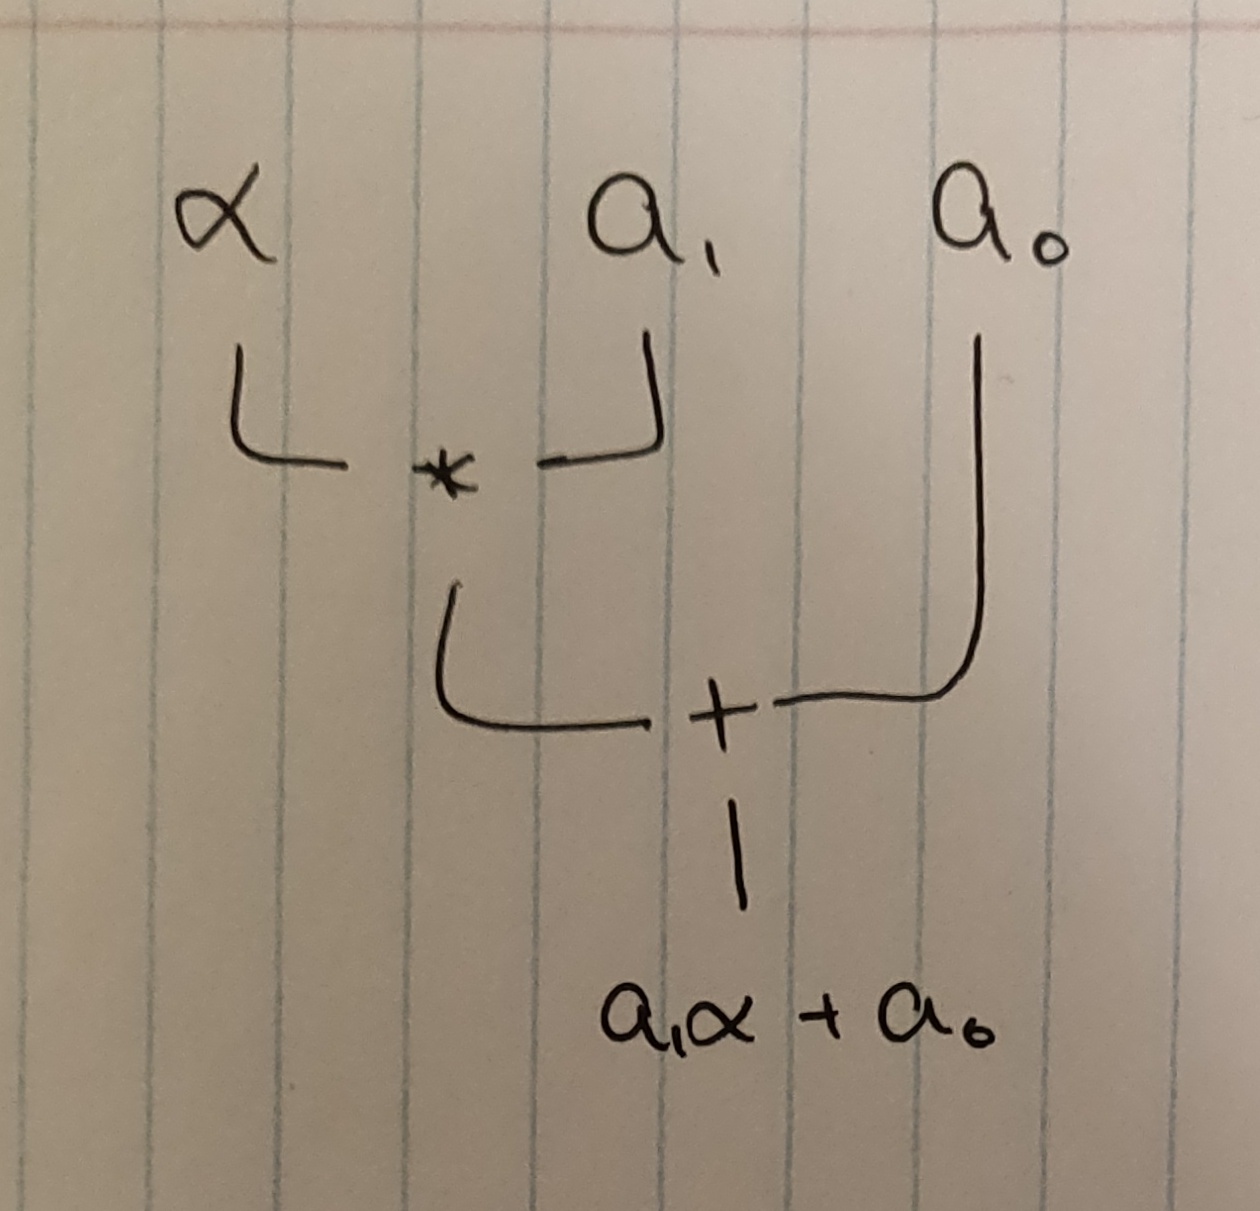
\includegraphics[width=0.8\textwidth]{images/lec4-circuit-1}
      \caption{A circuit representation of \\ $a_1\alpha + a_0$}
      \label{fig:lec4-circuit-1}
    \end{minipage}%
    \begin{minipage}{.5\textwidth}
      \centering
      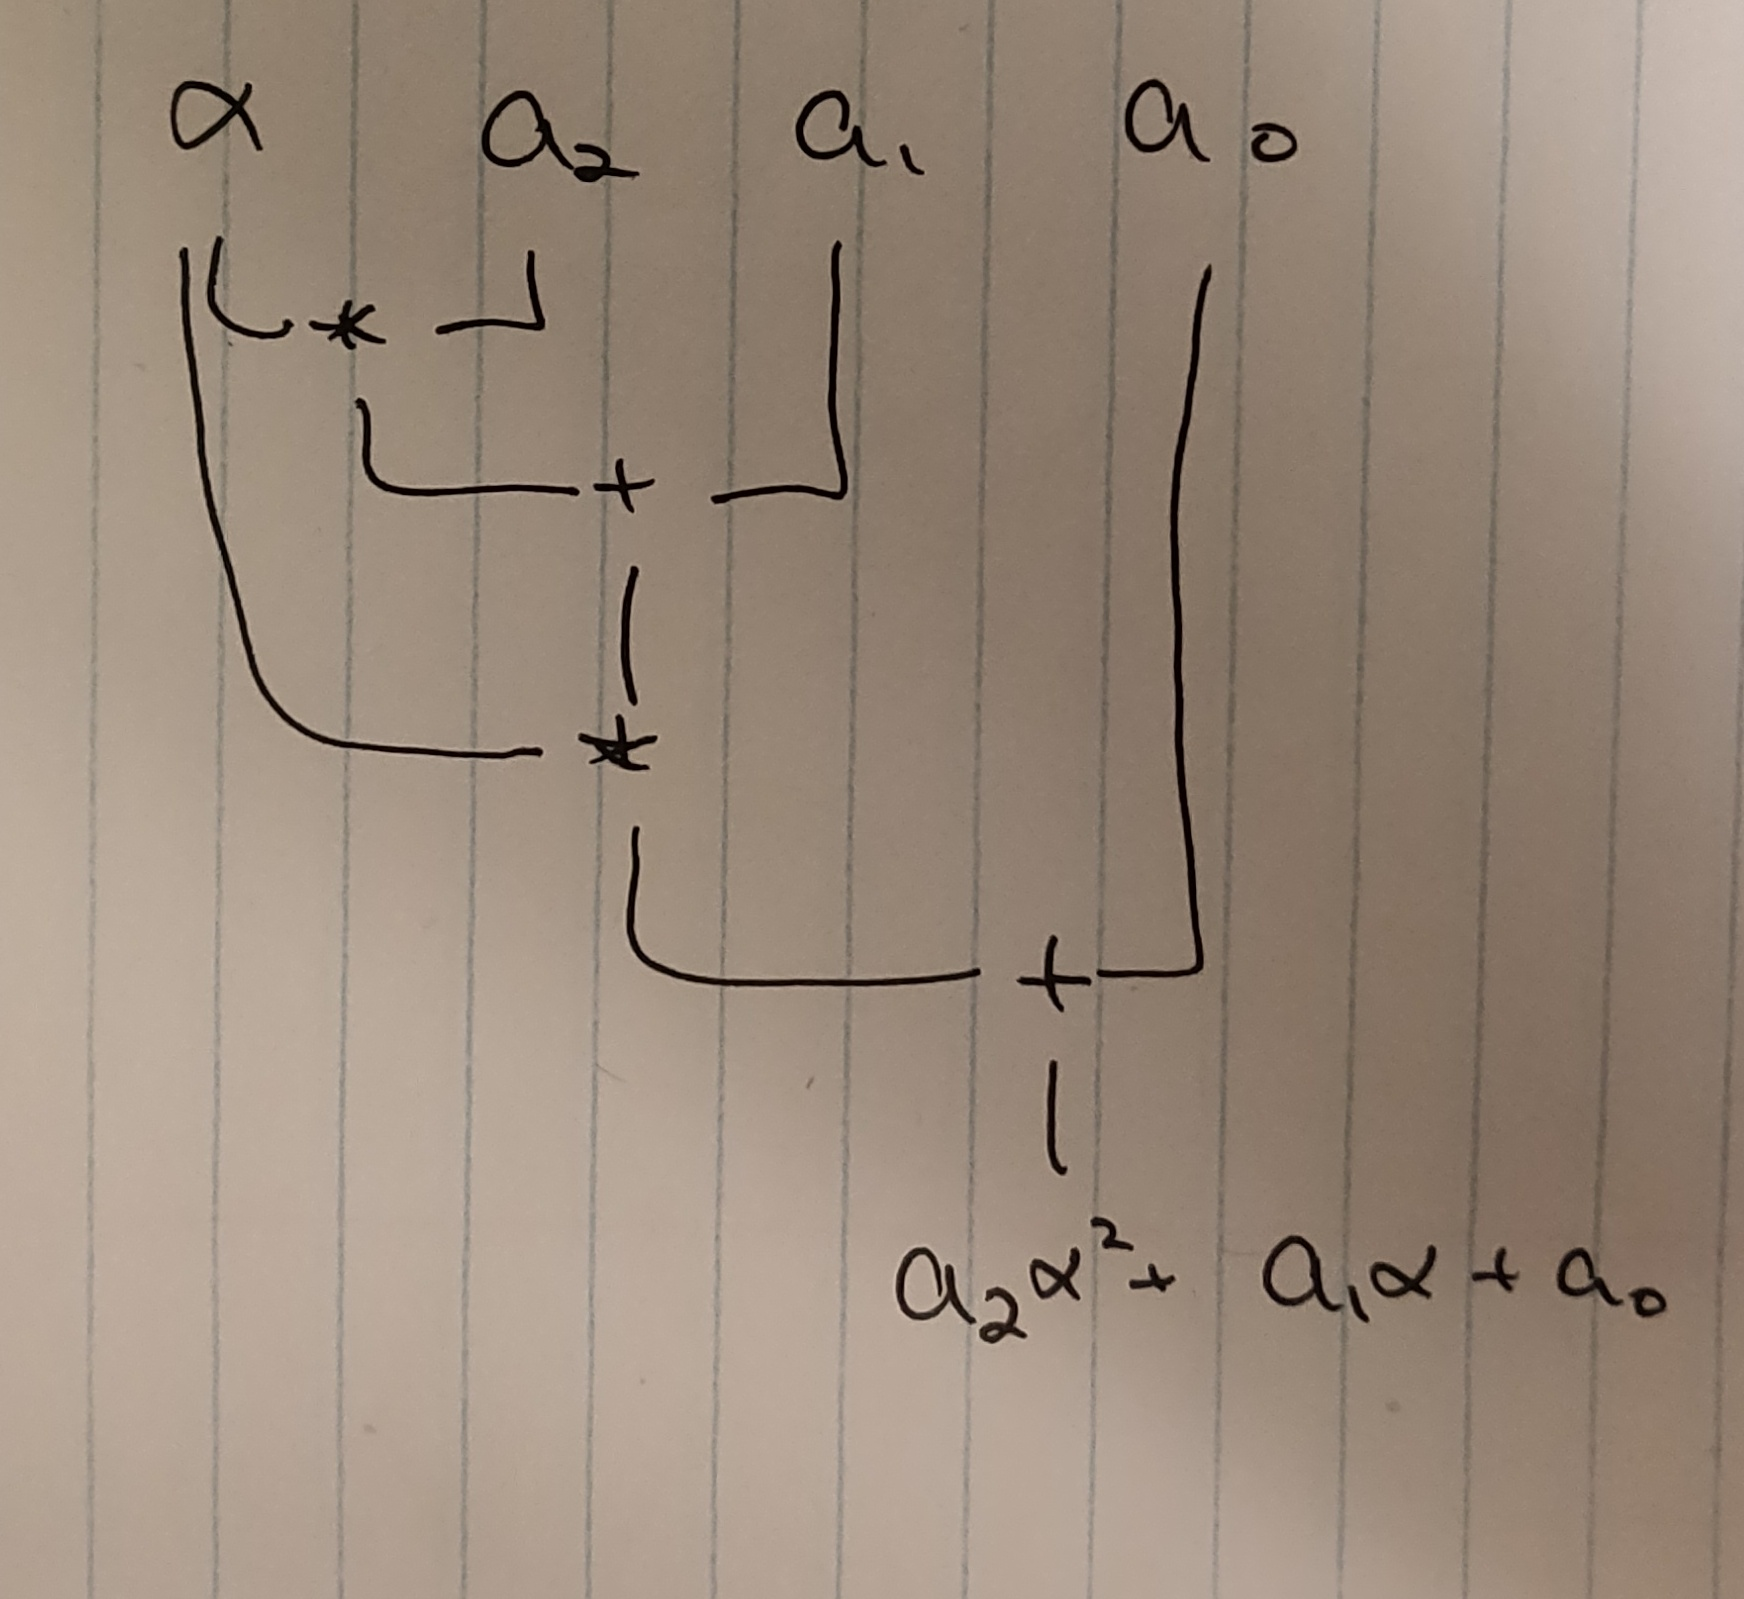
\includegraphics[width=0.8\textwidth]{images/lec4-circuit-2}
      \caption{{\footnotesize A circuit representation of \\ $a_2\alpha^2 + a_1\alpha + a_0$}}
      \label{fig:lec4-circuit-2}
    \end{minipage}
\end{figure}

\begin{remark}
    The depth of a circuit is the parallel complexity
\end{remark}